\problemname{Tight-Fit Sudoku}

At some point or another, most computer science students have written a standard Sudoku solving
program.  
% the original problem lacked a description of standard Sudoku so contestants not familiar
% with this puzzle would be left out.
In a standard Sudoku puzzle, a $9 \times 9$ grid that is partially filled in with digits is given.
The task is to complete the grid so that each digit occurs exactly once in every row, column,
and in each of $9$ $3 \times 3$ non-overlapping subregions marked in the grid.
This problem adds a slight twist to standard Sudoku to make it a bit more challenging.

Digits from $1$ to $9$ are entered in a $6 \times 6$ grid so that no number is repeated in any row, column 
or $3 \times 2$ outlined region as shown below. Some squares in the grid are split by a slash and need 
$2$ digits entered in them. The smaller number always goes above the slash.

\begin{figure}[!h]
\begin{center}
    \begin{tabular}{cc}
        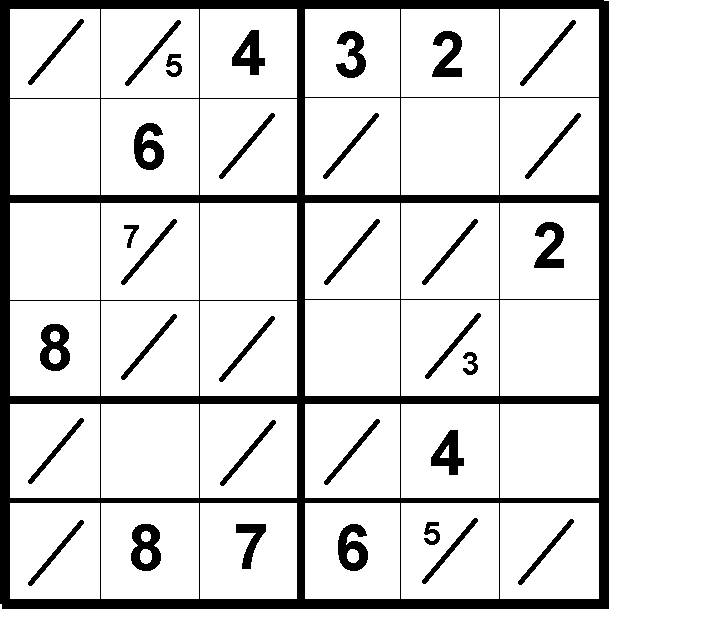
\includegraphics[width=.75\textwidth]{tfs-001.png} &
        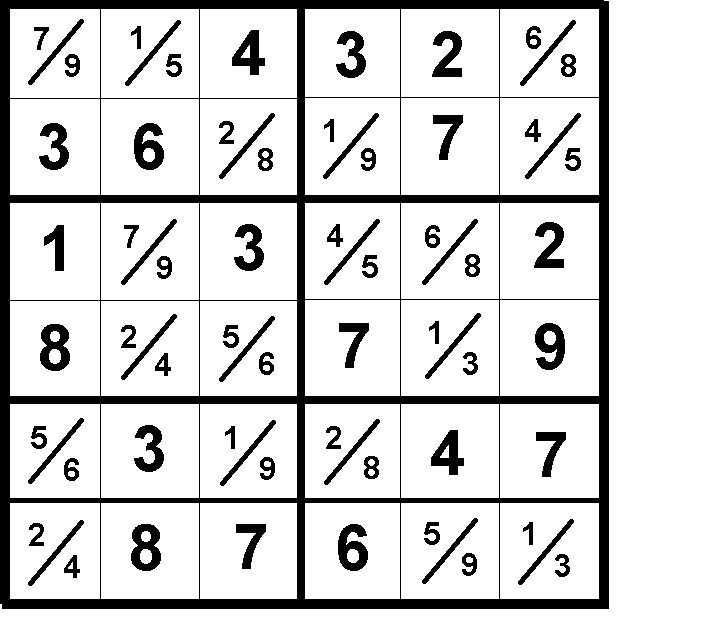
\includegraphics[width=.75\textwidth]{tfs-002.png} \\
        \textbf{Incomplete Grid} &
        \textbf{Solution Grid} \\
    \end{tabular}
\end{center}
\end{figure}

For this problem, you will write a program that takes as input an incomplete puzzle grid and outputs
the puzzle solution grid.

\section*{Input}

The input consists of a single data set.
This data set consists of $6$ lines of input
representing an incomplete Tight-Fit Sudoku grid. 
Each line has $6$ data elements, separated by spaces. 
A data element can be a digit (\texttt{1-9}), a dash (`\texttt{-}') 
for a blank square or two of these separated by a slash (`\texttt{/}').

\section*{Output}

Output $6$ lines showing the solution grid for the given input data set. Each line
will have $6$ data elements, separated by spaces. A data element can be a digit (\texttt{1-9}) 
or $2$ digits separated by a slash (`\texttt{/}').
The input will be chosen such that the solution grid is unique.
